\documentclass[10pt]{beamer}
\usetheme{Warsaw}
\usefonttheme[onlymath]{serif} 
\setbeamercovered{invisible}
\beamerdefaultoverlayspecification{<+->}

\usepackage[utf8]{inputenc}
\usepackage[english]{babel}
\usepackage[T1]{fontenc}
\usepackage{lmodern,amsmath,booktabs,setspace,mathtools,multicol}

\usepackage{hanging}% http://ctan.org/pkg/hanging
\setbeamertemplate{footnote}{%
	\hangpara{2em}{1}%
	\makebox[2em][l]{\insertfootnotemark}\footnotesize\insertfootnotetext\par%
}

\title{CS 280 Paper Presentation}
%\subtitle{Algorithm Design}
%\author[J. Kleinberg, E. Tardos]{Jon Kleinberg, \'{E}va Tardos}
\author{J Franco Ray}
\date{\today}

\begin{document}

\begin{frame}
	\maketitle
\end{frame}

\begin{frame}[noframenumbering]{Outline}
	\tableofcontents
\end{frame}

\section{Financial time series forecasting using support vector machines}
\subsection*{Introduction}
\begin{frame}{Financial time series forecasting}{using support vector machines}
	\textit{Kyoung-jae Kim, Dongguk University. 2013}
	\begin{itemize}[<1->]
		\item This study uses SVM to predict the stock price index
		\item Compared performance of SVM, ANN and case-based reasoning for stock market prediction
	\end{itemize}
\end{frame}
\begin{frame}{Introduction}{}
	\begin{itemize}[<1->]
		\item ANN has inconsistent performance when faced with noisy data and complex dimensionality
		\item Backprop algorithm still needs to determine several parameters such as input features, hidden layer size, learning rate and momentum term
		\item ANN implements the \textit{empirical risk minimization principle} while SVM implements the \textit{structural risk minimization principle}
	\end{itemize}
\end{frame}

\subsection*{Methodology}
\begin{frame}{Methodology}{}
	\begin{itemize}[<1->]
		\item Data used is technical indicators and direction of change in daily stock price index: 80\% for training, 20\% for validation
		\item There are 12 attributes that determine the direction of daily change, scaled into $\left[-1.0, 1.0\right]$ and classified to '0' or '1'
		\item Polynomial and RBF kernels are used for SVM; three-layer network for ANN and nearest-neighbor method for CBR to retrieve relevant cases
	\end{itemize}
	\footnotetext{Kyoung-jae Kim, Dongguk University. 2013}
\end{frame}
\begin{frame}{Methodology}
	\begin{block}{Why are the input values scaled into [-1, 1]?}<1->
		The goal of linear scaling is to independently normalize each feature component to ensure that larger values do not overwhelm smaller inputs to reduce prediction errors.
	\end{block}
\end{frame}
\begin{frame}{Methodology}{}
	\begin{figure}[H]
		\centering
		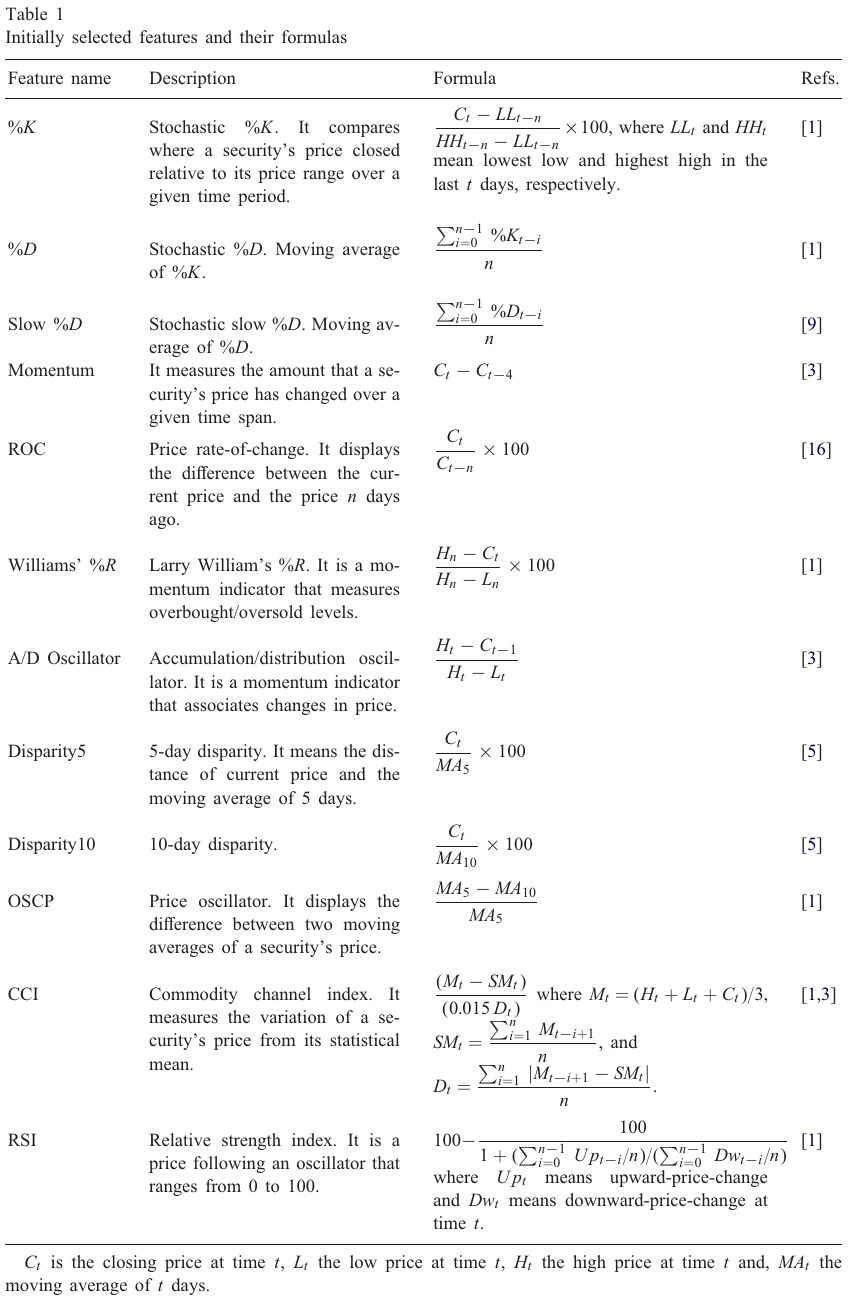
\includegraphics[width=0.45\textwidth]{stock0}
	\end{figure}
\end{frame}

\subsection*{Results}
\begin{frame}{Results}{}
	\begin{figure}[H]
		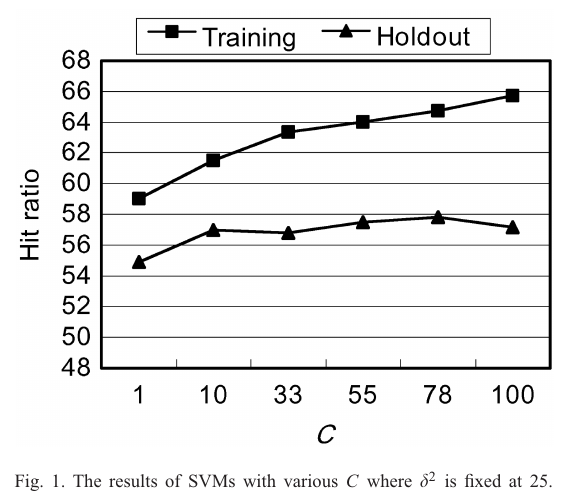
\includegraphics[width=0.5\textwidth]{stock1}
		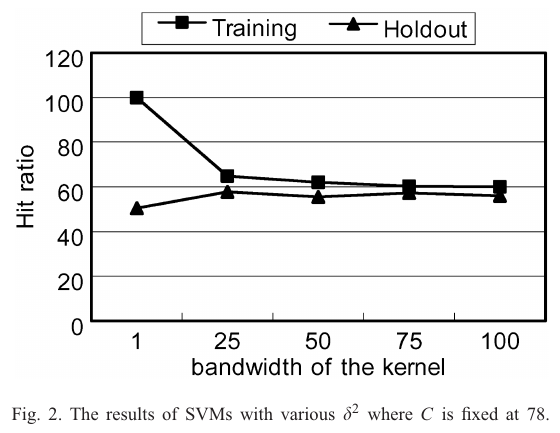
\includegraphics[width=0.5\textwidth]{stock2}
	\end{figure}
\end{frame}
\begin{frame}{Results}{}
	\begin{figure}[H]
		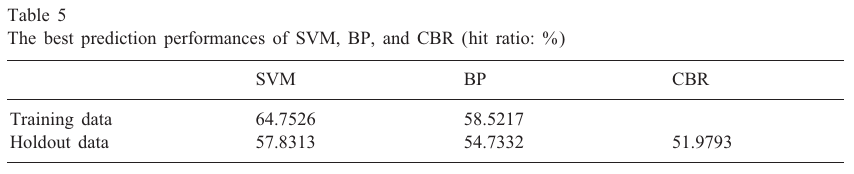
\includegraphics[width=\textwidth]{stock3}
	\end{figure}
	\begin{itemize}[<1->]
		\item SVM leads to better generalization than conventional techniques when used with optimal parameters
	\end{itemize}
\end{frame}

\section[Credit rating analysis with support vector machines and neural networks]{Credit rating analysis with support vector machines and neural networks: a market comparative study}
\subsection*{Introduction}
\begin{frame}{Credit rating analysis with support vector machines}{and neural networks: a market comparative study}
	\textit{Z. Huang, H. Chen, C. Hsu, W. Chen, S. Wu,\\ University of Arizona. 2003}
	\begin{itemize}[<1->]
		\item Used SVM, ANN and CBR to predict corporate credit ratings based on input financial variables
		\item Obtained relative importance of input variables fron the neural network models
		\item Conducted a market comparative analysis on the determining factors in US and Taiwan markets
	\end{itemize}
\end{frame}
\begin{frame}{Introduction}
	\begin{itemize}[<1->]
		\item Credit ratings is a measure of riskiness of bonds: lower rating indicates higher risk
		\item Typically very costly to obtain, needs large amount of time and human resources to perform deep analysis
		\item Rating agencies emphasize the importance of analysts' highly subjective judgment in determining credit ratings
	\end{itemize}
\end{frame}
\begin{frame}{Introduction}
	\begin{block}{Why are intelligent models important to credit rating analysis?}<1->
		It help users capture fundamental characteristics of different financial markets and which attributes have more contribution than others. In other terms, to reverse engineer the subjective judgment done by credit raters.
	\end{block}
\end{frame}
\subsection*{Methodology}
\begin{frame}{Methodology}
	\begin{columns}
		\begin{column}{0.5\textwidth}
			\begin{center}
				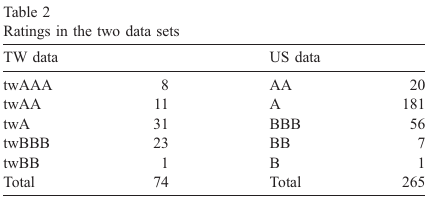
\includegraphics[width=\textwidth]{credit1}
			\end{center}
			\begin{itemize}
				\item Ran ANOVA on TW set to test whether differences between different rating classes were significant in each financial variable.
			\end{itemize}
		\end{column}
		\begin{column}{0.5\textwidth}
				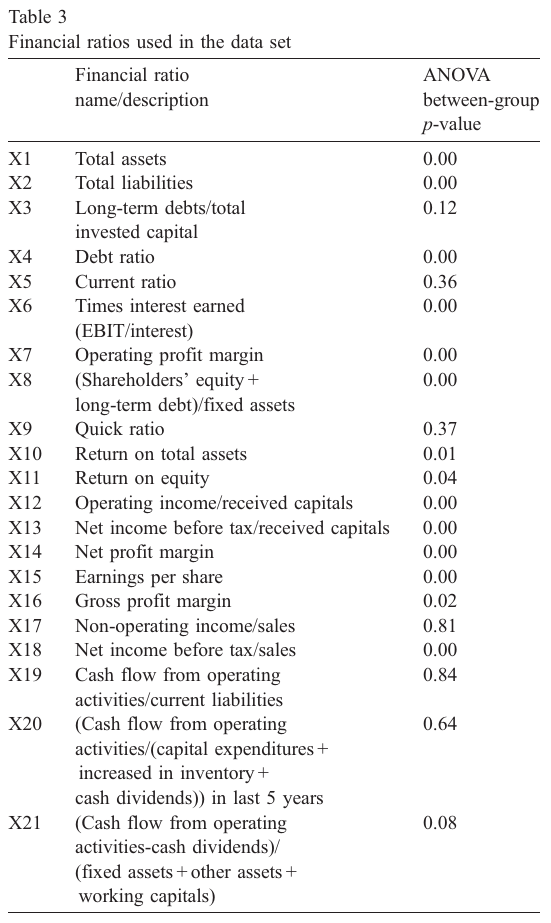
\includegraphics[width=.8\textwidth]{credit0}
		\end{column}
	\end{columns}
\end{frame}

\subsection*{Results}
\begin{frame}{Results}
	\begin{figure}
		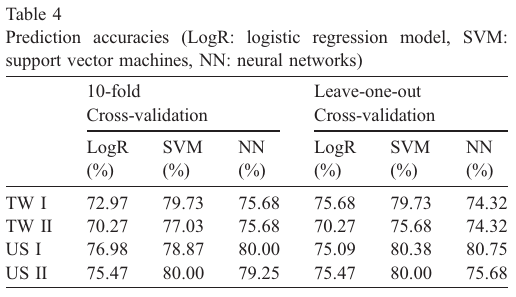
\includegraphics[width=.7\textwidth]{credit2}
	\end{figure}
	\begin{itemize}[<1->]
		\item Relatively small list of financial variables largely determined the rating results
	\end{itemize}
\end{frame}
\begin{frame}{Results}
	\begin{columns}
		\begin{column}{0.5\textwidth}
			\begin{center}
				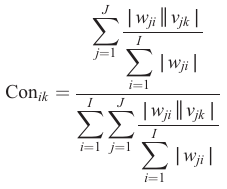
\includegraphics[width=.6\textwidth]{credit4}
			\end{center}
			\begin{itemize}[<1->]
				\item Garson's measure of relative contribution of input $i$ to output $k$
				\item Assessed relative importance of each input variables to the bond-rating process in different markets
			\end{itemize}
		\end{column}
		\begin{column}{0.5\textwidth}
			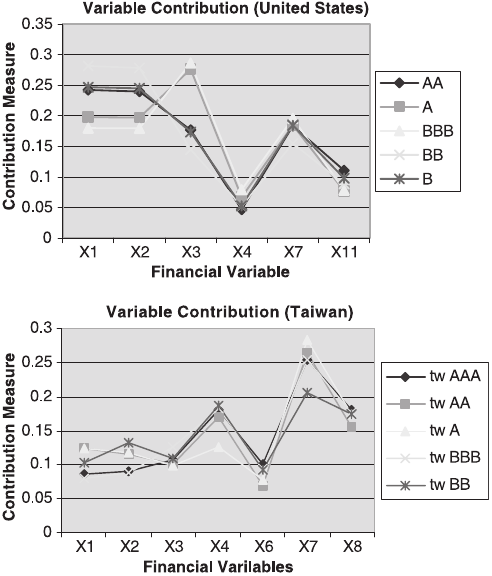
\includegraphics[width=\textwidth]{credit5}
		\end{column}
	\end{columns}
\end{frame}

\begin{frame}
	\begin{block}
		{
			\centering Thank you for your attention!
		}
	\end{block}
\end{frame}
\end{document}